% comments start with "%"

% define document
\documentclass{article}[12pt] 

% margin spacing
\usepackage[a4paper, margin=1in]{geometry}

% package imports
\usepackage{hyperref}   % for hyperlinks
\usepackage{xcolor}     % for color options
\usepackage{amsmath}    % for math notation
\usepackage{graphicx}   % for graphics/image attachments
\usepackage{tikz}       % for drawing graphics
\usepackage{float}      % for figure positioning

% hyperref setup (not required for demo)
\hypersetup{
    colorlinks=true,
    linkcolor=black,
    urlcolor=blue,
    citecolor=black,
    % pdfborderstyle={/S/U/W 1}
    }

% title setup
\title{Learning Notation: Introduction}
\author{
    Uppsala Pareto Seminars
    }
\date{03 March 2022}

% paragraph indent and spacing
\setlength{\parindent}{0pt}
\setlength{\parskip}{6pt}

\begin{document}
    
    \maketitle % create title
        
    \section*{Welcome} % first section
        
        Welcome to the Learning Notation mathematics seminars! The seminars are organized by economics masters students in Pareto to discuss mathematics and economics in an informal setting.
        
        Among others, we hope to venture topics including
        
        % make a list
        \begin{itemize}
            
            \item
            proof techniques and set theory,
            
            \item
            real analysis and advanced calculus,
            
            \item
            differential equations and linear algebra,
            
            \item
            probability theory,
            
            \item
            complex numbers and their geometry.
            
        \end{itemize}
        
        The motivation of the seminars is to provide a forum where we can discuss and explore mathematics without the stress and obligations of an academic class. The hope is that we can discover some of the beauty and rigor of mathematical ideas together.
        
        \begin{quote}
            \it
            A musician wakes from a terrible nightmare. In his dream he finds himself in a society where music education has been made mandatory. ... Since musicians are known to set down their ideas in the form of sheet music, these curious black dots and lines must constitute the “language of music”. It is imperative that students become fluent in this language if they are to attain any degree of musical competence; indeed, it would be ludicrous to expect a child to sing a song or play an instrument without having a thorough grounding in music notation and theory. Playing and listening to music, let alone composing an original piece, are considered very advanced topics and are generally put off until college, and more often graduate school. ...
            
            Waking up in a cold sweat, the musician realizes, gratefully, that it was all just a crazy dream. Of course! he reassures himself, ``No society would ever reduce such a beautiful and meaningful art form to something so mindless and trivial; no culture could be so cruel to its children as to deprive them of such a natural, satisfying means of human expression. How absurd!"
        \end{quote}
        \hfill -Paul Lockhart, \href{https://www.maa.org/external_archive/devlin/LockhartsLament.pdf}{\it A Mathematician's Lament}
        
        The name of the project, ``Learning Notation," comes from the idea that as daunting as mathematics can seem, it's just notation. Once you understand the notation, you understand the math.
        
        We have a \href{https://www.overleaf.com/4797466783cszvmfmgsbct}{shared Overleaf project} where we collaborate on \LaTeX{} notes for the seminars. We also have a \href{https://discord.gg/Atv2jfRZnx}{Discord server} for announcements and discussion and a \href{https://docs.google.com/spreadsheets/d/1Ge9dVUt8bkdbZr03XvqzWJXrUtmdrix6Oo6ylrGNNsM/edit?usp=sharing}{Google Sheet} for scheduling.
    
    
    % start second section
    \section*{How to use \LaTeX{}}
        
        \href{https://www.overleaf.com/learn/latex/Learn_LaTeX_in_30_minutes}{Overleaf} has great resources for learning how to use \LaTeX. This section also serves as a quick primer on using math notation with \LaTeX. See the \texttt{.tex} file for this document on Overleaf to see the \LaTeX code and comments. % hello!
    
    % subsection under the second section
    \section{Writing math symbols}
        
        In \LaTeX we can write in-line mathematical expressions alongside our text, for example: $\pi = 2\int_{-1}^{1}\sqrt{1 - x^2} \; dx \simeq 3.14159 $. \newline
        
    % start a subsection
    \subsection{Single-line equations}
    
        Using the \texttt{amsmath} package, we can also write single-line equations like so:
        \begin{equation}
            e^{i\pi} + 1 = 0.
        \end{equation}
        
        If we don't want the line numbers, we can use asterisks (*) to suppress them:
        \begin{equation*}
            1 + 2 = 3.
        \end{equation*}
    
    % start second subsection
    \subsection{Multi-line equations}
    
        We can also write multi-line equations.
        \begin{align}
            f(x) = a x^n, \; n \ge 2
            &\implies
            f'(x) = a n x^{n-1} \\  
            &\implies
            f''(x) = a n (n-1) x^{n-2}. \label{eqn:2nd-deriv}
        \end{align}
        
        We can reference a specific line in an equation. Here, equation \eqref{eqn:2nd-deriv} is the second derivative. If we don't want the line numbers, we can again suppress them.
        \begin{align*}
            a x^2 + b x + c = 0
            & \implies x^2 + p x + q = 0,
            \quad p = \frac{b}{a}, \; q = \frac{c}{a}, \; a \ne 0,
            \\
            & \implies x^2 + p x = -q
            \\
            & \implies x^2 + p x + \left(\frac{p}{2}\right)^2
            = -q + \left(\frac{p}{2}\right)^2
            \\
            & \implies \left( x + \frac{p}{2} \right)^2
            = \frac{p^2}{4} - q
            \\
            & \implies x + \frac{p}{2}
            = \pm \sqrt{ \frac{p^2}{4} - q }
            \\
            & \implies x
            = -\frac{p}{2} \pm \sqrt{ \frac{p^2}{4} - q }.
        \end{align*}
    
    \newpage
    
    % start second subsection
    \section{Text formatting}
        
        In \LaTeX{} you can format text, and also create lists:
        
        \begin{itemize}
            \item 
            \textit{Italics} (or {\it italics})
            
            \item
            \textbf{Bold} (or {\bf bold})
            
            \item
            \underline{Underline}
            
            \item
            \texttt{Command font}
            
        \end{itemize}
        
        We can create numbered lists also.
        
        \begin{enumerate}
            \item 
            Learn \LaTeX.
            
            \item
            Write master's thesis.
            
            \item
            Profit.
        \end{enumerate}
        
    
    
    % start third subsection
    \section{Tables}
        
        With \LaTeX{} we can create tables.
        \begin{table}[H] % position table "here"
            \centering
            \begin{tabular}{|c||c|c|} % row text alignment and vertical lines
                \hline % horizontal line
                   & A   & B \\
                 \hline\hline % double lines
                 C & 0.1 & 0.2 \\
                 \hline
                 D & 0.3 & 0.4 \\
                 \hline % horizontal line
            \end{tabular}
            \caption{Example Table} % caption
        \end{table}
        
        You can customize tables a lot.
        
        \begin{table}[H]
            \centering
            \caption{Social Media Use and GAD Symptoms during COVID-19}
            \setlength{\tabcolsep}{10pt}
            \renewcommand{\arraystretch}{.55}
            \setlength{\tabcolsep}{6pt}
            \renewcommand{\arraystretch}{.55}
            \begin{tabular}{lcccc}
                \hline
                 \\
                & \multicolumn{4}{c}{Symptoms of Moderate or Severe Generalized Anxiety Disorder}
                \\\\\hline\\
                & (1) & (2) & (3) & (4)
                \\\\\hline\\
                \multicolumn{2}{l}{\bf \textit{Use COVID-19 information from social media}} \\
                 \\
                Posts from news organizations & 0.070** & 0.069** & 0.025 & 0.0014 \\
                or magazines only & (0.030) & (0.028) & (0.023) & (0.035)\\
                 \\
                Posts from other users only
                 & 0.019 & 0.019 & -0.033 & 0.065 \\
                 & (0.028) & (0.027) & (0.030) & (0.045) \\
                 \\
                Posts from both sources & 0.078** & 0.084*** & 0.023 & 0.021 
                \\
                 & (0.031) & (0.031) & (0.031) & (0.041) \\
                \\
                \multicolumn{2}{l}{\bf \textit{Controls}} \\
                 \\
                Behavioural Controls & No & No & Yes & Yes \\
                 \\
                Demographic Controls & No & No & Yes & Yes \\
                 \\\\
                Observations & 3,961 & 3,495 & 3,397 & 3,397 \\
                 \\
                R-squared & 0.010 & 0.039 & 0.243 & 0.095 \\\\ \hline
                 \\
                \multicolumn{5}{c}{ Robust standard errors in parentheses} \\
                \multicolumn{5}{c}{ *** p$<$0.01, ** p$<$0.05, * p$<$0.1} \\
                \\ \hline
            \end{tabular}
        \end{table}
        
    \section{Graphics}
    
        We can create graphics also,
        \begin{figure}[H] % position graphic "here"
            \centering
            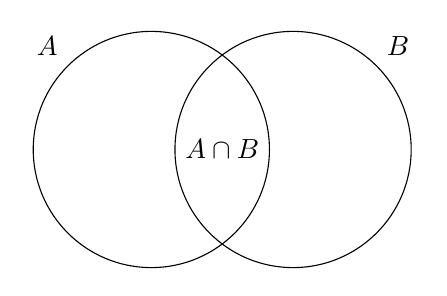
\begin{tikzpicture}
                % Set A
                \node [draw,
                    circle,
                    minimum size =3cm,
                    label={135:$A$}] (A) at (0,0){};
                % Set B
                \node [draw,
                    circle,
                    minimum size =3cm,
                    label={45:$B$}] (B) at (1.8,0){};
                % Set intersection label
                \node at (0.9,0) {$A\cap B$};
            \end{tikzpicture}
            \caption{Venn diagram}
        \end{figure}
        
        and attach images as graphic figures.
        \begin{figure}[H]
            \centering
            % set width of graphic in-line with text
            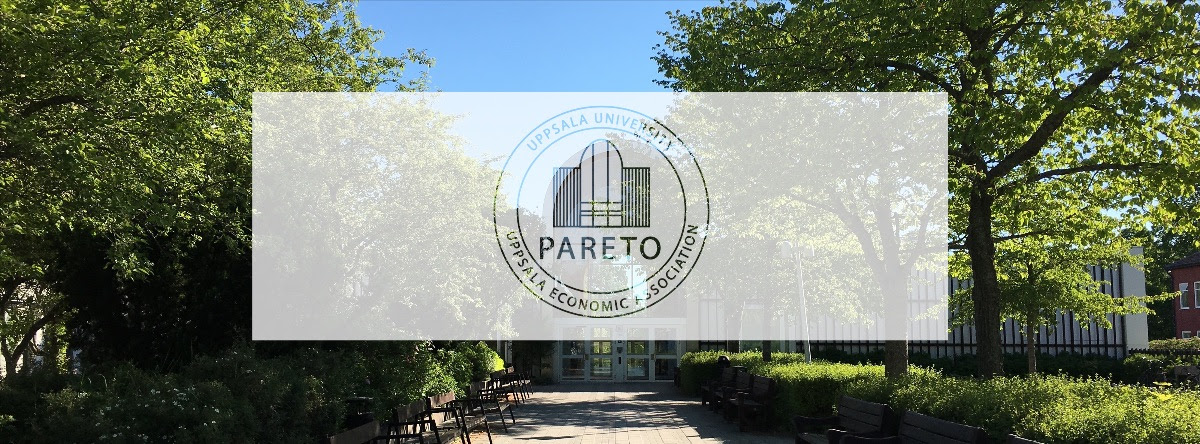
\includegraphics[width=\textwidth]{attachments/0-pareto.jpg}
            \caption{Pareto logo}
        \end{figure}
        
        Document wise, \LaTeX{} can do pretty much anything. There's a lot to learn, but everything is just a Google search away.
        
    
    \section{Bibliography}
        
        If we use citations, we can create a bibliography. \cite{doe22}
        
        \begin{quote}
            \emph{``Simplicity is the final achievement. After one has played a vast quantity of notes and more notes, it is simplicity that emerges as the crowning reward of art."}
        \end{quote}
        \hfill - Frédéric Chopin \cite{chopin}


        % choose the "plain" reference style
        \bibliographystyle{plain}
        
        % entries are in the .bib file
        \bibliography{bibs/0-intro.bib}


\end{document}